% ------------------------------------------------------------------------
% file `ad-complogic-report-exercise-4-solution-body.tex'
%
%     solution of type `exercise' with id `4'
%
% generated by the `solution' environment of the
%   `xsim' package v0.10 (2017/09/19)
% from source `ad-complogic-report' on 2017/11/26 on line 270
% ------------------------------------------------------------------------
^^I^^IНехай задана перемикальна функція $f(x_1, x_2, x_3, x_4)$, тоді побудуємо таблицю істинності~(табл.~\ref{tab:task4-function-truth-table}) за діаграмою Вейча заданої функції~(рис.~\ref{fig:task4-veitch-diagram}).
^^I^^I
^^I^^I\begin{table}[!htbp]
^^I^^I\centering
^^I^^I^^I\begin{tabular}{ccccc}
^^I^^I^^I^^I\toprule
^^I^^I^^I^^I^^I$x_1$ & $x_2$ & $x_3$ & $x_4$ & $f(x_1, x_2, x_3, x_4)$ \\
^^I^^I^^I^^I\midrule
^^I^^I^^I^^I^^I0     & 0     & 0     & 0     & 0 \\
^^I^^I^^I^^I^^I0     & 0     & 0     & 1     & 0 \\
^^I^^I^^I^^I^^I0     & 0     & 1     & 0     & 0 \\
^^I^^I^^I^^I^^I0     & 0     & 1     & 1     & 0 \\
^^I^^I^^I^^I^^I0     & 1     & 0     & 0     & 1 \\
^^I^^I^^I^^I^^I0     & 1     & 0     & 1     & — \\
^^I^^I^^I^^I^^I0     & 1     & 1     & 0     & 1 \\
^^I^^I^^I^^I^^I0     & 1     & 1     & 1     & — \\
^^I^^I^^I^^I^^I1     & 0     & 0     & 0     & 0 \\
^^I^^I^^I^^I^^I1     & 0     & 0     & 1     & 1 \\
^^I^^I^^I^^I^^I1     & 0     & 1     & 0     & — \\
^^I^^I^^I^^I^^I1     & 0     & 1     & 1     & 0 \\
^^I^^I^^I^^I^^I1     & 1     & 0     & 0     & 1 \\
^^I^^I^^I^^I^^I1     & 1     & 0     & 1     & 1 \\
^^I^^I^^I^^I^^I1     & 1     & 1     & 0     & 0 \\
^^I^^I^^I^^I^^I1     & 1     & 1     & 1     & — \\
^^I^^I^^I^^I\bottomrule
^^I^^I^^I\end{tabular}
^^I^^I\caption{Таблиця істинності заданої функції $f(x_1, x_2, x_3, x_4)$}
^^I^^I\label{tab:task4-function-truth-table}
^^I^^I\end{table}
^^I^^I
^^I^^I% Запишемо функцію у вигляді досконалої диз'\-юн\-ктив\-ної нормальної форми (ДДНФ) двійкових представлень.
^^I^^IЗапишемо функцію у вигляді досконалої диз'\-юн\-ктив\-ної нормальної форми двійкових представлень.
^^I^^I\[
^^I^^I^^If(x_1, x_2, x_3, x_4) = 0100 \lor 0110 \lor 1001 \lor 1100 \lor 1101.
^^I^^I\]
^^I^^I
^^I^^IСкладемо таблицю мінтермів~(табл.~\ref{tab:task4-minterm-table}). Для виконання мінімізації внесемо до неї не тільки мінтерми, а й терми, значення яких нас не цікавить (\langdef{англ.}{don't-care terms}).
^^I^^I
^^I^^I\begin{table}[!htbp]
^^I^^I\centering
^^I^^I^^I\begin{tabular}{v{5em}ln{7em}}
^^I^^I^^I^^I\toprule
^^I^^I^^I^^I^^IКількість одиниць & Мінтерм & Двійкове представлення\\
^^I^^I^^I^^I\midrule
^^I^^I^^I^^I^^I1           & \texttt{m04}      & \texttt{0100}\\
^^I^^I^^I^^I^^I\cmidrule(lr){1-3}
^^I^^I^^I^^I^^I\multirow{5}{*}{2}
^^I^^I^^I^^I^^I            & \texttt{m06}      & \texttt{0110}\\
^^I^^I^^I^^I^^I            & \texttt{m09}      & \texttt{1001}\\
^^I^^I^^I^^I^^I            & \texttt{m12}      & \texttt{1100}\\
^^I^^I^^I^^I^^I            & \texttt{d05}      & \texttt{0101}\\
^^I^^I^^I^^I^^I            & \texttt{d10}      & \texttt{1010}\\
^^I^^I^^I^^I^^I\cmidrule(lr){1-3}
^^I^^I^^I^^I^^I\multirow{2}{*}{3}
^^I^^I^^I^^I^^I            & \texttt{m13}      & \texttt{1101}\\
^^I^^I^^I^^I^^I            & \texttt{d07}      & \texttt{0111}\\
^^I^^I^^I^^I^^I\cmidrule(lr){1-3}
^^I^^I^^I^^I^^I4           & \texttt{d15}      & \texttt{1111}\\
^^I^^I^^I^^I\bottomrule
^^I^^I^^I\end{tabular}
^^I^^I\caption{Таблиця мінтермів}
^^I^^I\label{tab:task4-minterm-table}
^^I^^I\end{table}
^^I^^I
^^I^^IПобудуємо таблицю для пошуку простих імплікант~(табл.~\ref{tab:task4-finding-prime-implicants}). Прості імпліканти виділені жирним шрифтом.
^^I^^I
^^I^^I\begin{table}[!htbp]
^^I^^I\centering
^^I^^I^^I\begin{tabular}{v{5em}cccccc}
^^I^^I^^I^^I\toprule
^^I^^I^^I^^I^^IКількість одиниць & Мінтерм & & \multicolumn{2}{c}{2-імпліканти} & \multicolumn{2}{c}{4-імпліканти}\\
^^I^^I^^I^^I\midrule
^^I^^I^^I^^I^^I\multirow{3}{*}{1}
^^I^^I^^I^^I^^I^^I& \texttt{m04}          & \texttt{0100}          & \texttt{(m04,m06)}          & \texttt{01—0}          & \strong{\texttt{(m04,m06,d05,d07)}} & \strong{\texttt{01——}}\\
^^I^^I^^I^^I^^I^^I&                       &                        & \texttt{(m04,m12)}          & \texttt{—100}          & \strong{\texttt{(m04,m12,m13,d05)}} & \strong{\texttt{—10—}}\\
^^I^^I^^I^^I^^I^^I&                       &                        & \texttt{(m04,d05)}          & \texttt{010—}          &                                     &  \\
^^I^^I^^I^^I^^I\cmidrule(lr){1-7}
^^I^^I^^I^^I^^I\multirow{6}{*}{2}
^^I^^I^^I^^I^^I^^I& \texttt{m06}          & \texttt{0110}          & \texttt{(m06,d07)}          & \texttt{011—}          & \strong{\texttt{(m13,d05,d07,d15)}} & \strong{\texttt{—1—1}}\\
^^I^^I^^I^^I^^I^^I& \texttt{m09}          & \texttt{1001}          & \strong{\texttt{(m09,m13)}} & \strong{\texttt{1—01}} &                                     & \\
^^I^^I^^I^^I^^I^^I& \texttt{m12}          & \texttt{1100}          & \texttt{(m12,m13)}          & \texttt{110—}          &                                     & \\
^^I^^I^^I^^I^^I^^I& \texttt{d05}          & \texttt{0101}          & \texttt{(d05,m13)}          & \texttt{—101}          &                                     & \\
^^I^^I^^I^^I^^I^^I&                       &                        & \texttt{(d05,d07)}          & \texttt{01—1}          &                                     & \\
^^I^^I^^I^^I^^I^^I& \strong{\texttt{d10}} & \strong{\texttt{1010}} &                             &                        &                                     & \\
^^I^^I^^I^^I^^I\cmidrule(lr){1-7}
^^I^^I^^I^^I^^I\multirow{2}{*}{3}
^^I^^I^^I^^I^^I^^I& \texttt{m13}          & \texttt{1101}          & \texttt{(m13,d15)}          & \texttt{11—1}          &                                     & \\
^^I^^I^^I^^I^^I^^I& \texttt{d07}          & \texttt{0111}          & \texttt{(d07,d15)}          & \texttt{—111}          &                                     & \\
^^I^^I^^I^^I^^I\cmidrule(lr){1-7}
^^I^^I^^I^^I^^I\multirow{1}{*}{4}
^^I^^I^^I^^I^^I^^I& \texttt{d15}          & \texttt{1111}          &                             &                        &                                     & \\
^^I^^I^^I^^I\bottomrule
^^I^^I^^I\end{tabular}
^^I^^I\caption{Таблиця пошуку простих імплікант}
^^I^^I\label{tab:task4-finding-prime-implicants}
^^I^^I\end{table}
^^I^^I
^^I^^IСкладаємо таблицю простих імплікант (табл.~\ref{tab:task4-coverage-table}). До неї заносимо лише ті виходи функції, які мають значення. Ядрами будуть ті значення, у рядках яких існує лише одне перекриття.
^^I^^I
^^I^^I\begin{table}[!htbp]
^^I^^I\centering
^^I^^I^^I\begin{tabular}{lcccc}
^^I^^I^^I^^I\toprule
^^I^^I^^I^^I^^I& \texttt{01——} & \texttt{—10—} & \texttt{—1—1} & \texttt{1—01} \\
^^I^^I^^I^^I\midrule
^^I^^I^^I^^I\texttt{m04}  &  \xmark       & \xmark        &               &               \\
^^I^^I^^I^^I\texttt{m06}  &  \xmarkbf     &               &               &               \\
^^I^^I^^I^^I\texttt{m09}  &               &               &               & \xmarkbf      \\
^^I^^I^^I^^I\texttt{m12}  &               & \xmarkbf      &               &               \\
^^I^^I^^I^^I\texttt{m13}  &               & \xmark        & \xmark        & \xmark        \\
^^I^^I^^I^^I\bottomrule
^^I^^I^^I\end{tabular}
^^I^^I\caption{Таблиця покриття}
^^I^^I\label{tab:task4-coverage-table}
^^I^^I\end{table}
^^I^^I
^^I^^IТаким чином за методом Квайна\nbspthin —\nbspthin МакКласкі отримали МДНФ такого вигляду:
^^I^^I\[
^^I^^I^^If (x_1, x_2, x_3, x_4) = x_1 \land \neg{x_3} \land x_4 \lor x_2 \land \neg{x_3} \lor \neg{x_1} \land x_2.
^^I^^I\]
^^I^^I
^^I^^IПереходимо у базис АБО—НЕ:
^^I^^I\begin{IEEEeqnarray*}{rCl}
^^I^^I^^If (x_1, x_2, x_3, x_4) &=& x_1 \land \neg{x_3} \land x_4 \lor x_2 \land \neg{x_3} \lor \neg{x_1} \land x_2\\
^^I^^I^^I                       &=& (\neg{x_1} \lnor \neg{x_3}) \lnor (x_1 \lnor x_2) \lnor (x_2 \lnor x_4).
^^I^^I\end{IEEEeqnarray*}
^^I^^I
^^I^^IРеалізуємо отриману перемикальну функцію~(рис.~\ref{fig:task4-schematic}).
^^I^^I
^^I^^I\begin{figure}[!htbp]
^^I^^I\centering
^^I^^I^^I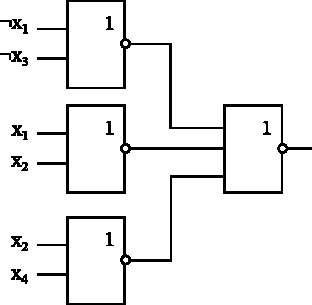
\includegraphics[]{task4-schematic.pdf}
^^I^^I\caption{Схема отриманої перемикальної функції}
^^I^^I\label{fig:task4-schematic}
^^I^^I\end{figure}
^^I^^I
